%15 min preso!
\documentclass[xcolor=table,aspectratio=169]{beamer}
\usepackage{beamerthemesplit}
\usepackage{wrapfig}
\usetheme{SPbGU}
\usepackage{pdfpages}
\usepackage{amsmath}
\usepackage{cmap}
\usepackage[T2A]{fontenc}
\usepackage[utf8]{inputenc}
\usepackage[english]{babel}
\usepackage{indentfirst}
%\usepackage{amsmath}
\usepackage{newtxmath}
\usepackage{tikz}
\usepackage{multirow}
\usepackage[noend]{algpseudocode}
\usepackage{algorithm}
\usepackage{algorithmicx}
\usepackage{fancyvrb}
\usepackage{hyperref}
\usepackage{nicematrix}
\definecolor{links}{HTML}{2A1B81}
\hypersetup{colorlinks,linkcolor=,urlcolor=links}
\usetikzlibrary{calc}
\usetikzlibrary{shapes, backgrounds}
\usetikzlibrary{arrows,automata}
\usetikzlibrary{positioning}
\usetikzlibrary{fit}
\usetikzlibrary{shapes.callouts}
\usetikzlibrary{shapes.misc}
\usepackage{xparse}
\usepackage{fontawesome}

\usepackage{etoolbox,refcount}
\usepackage{multicol}

\usepackage{tabularx}
\newcolumntype{Y}{>{\raggedleft\arraybackslash}X}

\renewcommand{\thealgorithm}{}

\newtheorem{mytheorem}{Theorem}
\renewcommand{\thealgorithm}{}

\newcommand{\tikzmark}[1]{\tikz[overlay,remember picture] \node (#1) {};}
\def\Put(#1,#2)#3{\leavevmode\makebox(0,0){\put(#1,#2){#3}}}

\newcommand{\ltz}{$< 1$}

\tikzset{
    state/.style={
           rectangle,
           rounded corners,
           draw=black, very thick,
           minimum height=2em,
           inner sep=2pt,
           text centered,
           },
}

\tikzset{
    invisible/.style={opacity=0,text opacity=0},
    visible on/.style={alt=#1{}{invisible}},
    alt/.code args={<#1>#2#3}{%
      \alt<#1>{\pgfkeysalso{#2}}{\pgfkeysalso{#3}} % \pgfkeysalso doesn't change the path
    },
}

\tikzset{cross/.style={cross out, draw=black, minimum size=2*(#1-\pgflinewidth), inner sep=0pt, outer sep=0pt, ultra thick},
%default radius will be 1pt. 
cross/.default={1pt}}

\NewDocumentCommand{\mycallout}{r<> O{opacity=0.8,text opacity=1} m m m}{%
\tikz[remember picture, overlay]\node[align=center, fill=cyan!20, text width=#5cm,
#2,visible on=<#1>, rounded corners,
draw,rectangle callout,anchor=pointer,callout relative pointer={(290:0.5cm)}]
at (#3) {#4};
}

\NewDocumentCommand{\mycalloutR}{r<> O{opacity=0.8,text opacity=1} m m m}{%
\tikz[remember picture, overlay]\node[align=center, fill=cyan!20, text width=#5cm,
#2,visible on=<#1>, rounded corners,
draw,rectangle callout,anchor=pointer,callout relative pointer={(30:0.8cm)}]
at (#3) {#4};
}

\newcommand\colR{\cellcolor{red!20}}
\newcommand\colB{\cellcolor{blue!20}}
\newcommand\colG{\cellcolor{green!20}}
\definecolor{Gray}{gray}{0.8}

%callout relative pointer={(230:0.5cm)}]

\newcounter{countitems}
\newcounter{nextitemizecount}
\newcommand{\setupcountitems}{%
  \stepcounter{nextitemizecount}%
  \setcounter{countitems}{0}%
  \preto\item{\stepcounter{countitems}}%
}
\makeatletter
\newcommand{\computecountitems}{%
  \edef\@currentlabel{\number\c@countitems}%
  \label{countitems@\number\numexpr\value{nextitemizecount}-1\relax}%
}
\newcommand{\nextitemizecount}{%
  \getrefnumber{countitems@\number\c@nextitemizecount}%
}
\newcommand{\previtemizecount}{%
  \getrefnumber{countitems@\number\numexpr\value{nextitemizecount}-1\relax}%
}
\makeatother    
\newenvironment{AutoMultiColItemize}{%
\ifnumcomp{\nextitemizecount}{>}{3}{\begin{multicols}{2}}{}%
\setupcountitems\begin{itemize}}%
{\end{itemize}%
\unskip\computecountitems\ifnumcomp{\previtemizecount}{>}{3}{\end{multicols}}{}}


\beamertemplatenavigationsymbolsempty

%%%%%%% 40 минут доклад %%%%%%%%%
%GraphBLAS предлагает разреженную линейную алгебру как путь к высокопроизводительному (параллельному) анализу графов. 
%Попробуем поглубже познакомиться с таким подходом. Начнём разговор с рассмотрения базовых связей между задачами анализа 
%графов и линейной алгеброй. Обсудим, как может быть устроена параметризация операций над матрицами и векторами, и причём тут полукольца. 
%Посмотрим на то, как в рамках линейной алгебры можно учитывать не только топологию графа, но атрибуты вершин и рёбер.
%В финале поговорим о том, каких успехов уже удалось добиться мировому сообществу на пути трансляции привычных языков запросов в операции линейной алгебры, 
%и каковы сейчас основные направления развития в этой области.

\title[Линейная алгебра и запросы к графам]{Линейная алгебра как основа для языка запросов к графам}
\institute[СПбГУ]{
Санкт-Петербургский Государственный Университет
}

\author[Семён Григорьев]{Семён Григорьев}

\date{09 декабря 2025}

\begin{document}
{
\begin{frame}[fragile]
  \begin{table}
  \centering  
  \begin{tabularx}{\linewidth}{XcX}
    \hfill
    & 
    & \hfill \includegraphics[height=1.4cm]{pictures/SPbSU_Logo.pdf}
  \end{tabularx}
  \end{table}
  \titlepage
\end{frame}
}

\begin{frame}[fragile]
  \frametitle{Семён Григорьев}
  \begin{minipage}{0.70\textwidth}
  \begin{itemize}    
    \item Доцент кафедры системного программирования Санкт-Петербургского Государственного Университета
    %\item Научный сотрудник лаборатории YADRO
    \item Руководитель исследовательской группы
    \item Области интересов
    \begin{itemize}
      \item \textbf{Высокопроизводительная линейная алгебра} для анализа графов
      \begin{itemize}
        \item \textbf{Обобщённая}: матрицы и вектора параметризованы типом элемента, операции над ними могут быть заданы пользователем
        \item \textbf{Разреженная}: специализированные структуры для хранения матриц и векторов, специализированные алгоритмы для их обработки 
        \item В том числе, с использованием \textbf{графических ускорителей}
      \end{itemize}
      \item \textbf{Высокопроизводительный анализ графов}      
    \end{itemize}
    \end{itemize}
\end{minipage}
\begin{minipage}[t]{0.29\textwidth}
  \begin{center}
\includegraphics[width=0.8\textwidth]{pictures/SemyonGrigorev.jpg}
  \end{center}
  {\scriptsize
\begin{itemize}    
  \item Email: s.v.grigoriev@mail.spbu.ru
  \item GitHub: \href{https://github.com/gsvgit}{gsvgit}
  \item Google Scholar: \href{https://scholar.google.com/citations?hl=ru&user=kP4dqUAAAAAJ&view_op=list_works&sortby=pubdate}{Semyon Grigorev}
  \item DBLP: \href{https://dblp.org/pid/181/9903.html}{Semyon V. Grigorev}
\end{itemize}
  }
\end{minipage}
\end{frame}

\begin{frame}[fragile]
  \frametitle{GraphBLAS\footnote{\url{https://graphblas.org/}}}
  \begin{itemize}
    \item API для создания алгоритмов анализа графов на основе линейной алгебры 
    \begin{itemize}
      \item Различные операции над матрицами и векторами (\underline{\textbf{разреженными}})
      \item Параметризация алгебраическими структурами: полукольцами, моноидами и т.д.
    \end{itemize}
    \item Позволяет выражать \underline{\textbf{различные}} алгоритмы
    \begin{itemize}
      \item Обход в ширину, поиск кратчайших путей, достижимость, \ldots
      \item Подсчёт треугольников, PageRank, остовные деревья, кластеризация, \ldots
      \item Навигационные запросы: \textbf{RPQ, CFPQ,} \ldots
    \end{itemize}
    \item Подробнее
    \begin{itemize}
      \item The GraphBLAS C API Specification\footnote{\url{https://graphblas.org/docs/GraphBLAS_API_C_v2.1.0.pdf}}
      \item GraphBLAS Pointers\footnote{\url{https://graphblas.org/GraphBLAS-Pointers/}}
      \item \textbf{SuiteSparse:GraphBLAS}\footnote{\url{https://github.com/DrTimothyAldenDavis/GraphBLAS}} --- \underline{\textbf{эталон}} на чистом C
      \item \textbf{LAGraph}\footnote{\url{https://github.com/GraphBLAS/LAGraph}} --- коллекция прикладных алгоритмов анализа графов
    \end{itemize}
    \end{itemize}
\end{frame}

\begin{frame}[fragile]
  \frametitle{Отношения и матрицы}
  $$ |S_A| = n, |S_B| = k, |S_C| = m$$
  $$\mathcal{N_A}: [0\ldots (n-1)] \to S_A$$, биекция
  $$R_1 \subseteq S_A \times S_B$$
  $$R_2 \subseteq S_B \times S_C$$
  $$R_3 = \{ (x,z) \mid (x,y) \in R_1, (y,z) \in R_2 \}$$
  $$M_{n \times k}^{R_1}: M[i,j] = 1 \iff (\mathcal{N_A}(i),\mathcal{N_B}(j)) \in R_1; \text{иначе } M[i,j] = 0$$
  $$M_{k \times m}(R_2): M[i,j] = 1 \iff ; \text{иначе } M[i,j] = 0$$
  $$M_{n \times m}(R_3) = M(R_1) \times M(R_2)$$
\end{frame}


\begin{frame}[fragile]
  \frametitle{Полукольца}
  $$ C = A \times B $$
  $$ C[i,j] = \sum_{k=0}^{n-1} A[i,k] * B[k,j] $$
  $$A: \texttt{Matrix}\langle T_1 \rangle $$
  $$B: \texttt{Matrix} \langle T_2 \rangle$$
  $$C: \texttt{Matrix}\langle T_3 \rangle$$
  $$\otimes: T_1 \times T_2 \to T_3$$
  $$\oplus: T_3 \times T_3 \to T_3$$
  $$\vmathbb{0}: T_3$$

  \NiceMatrixOptions{code-for-first-row = \color{red},
                     code-for-first-col = \color{blue},
                     code-for-last-row = \color{red},
                     code-for-last-col = \color{blue}}
$$
\begin{pNiceArray}{cccc}[first-col,last-col,nullify-dots]
  &  & \Cdots &  &  & \\
i & a_{i0} & \Cdots & & a_{i(k-1)} & i \\
  &  & \Cdots &  &  & \\
  &  & \Cdots &  &  & 
\end{pNiceArray}
\times
\begin{pNiceArray}{cccc}[first-row,last-row=5,nullify-dots]
 & & j &                             \\
   &              & b_{0j} &         \\
  \Vdots & \Vdots & \Vdots & \Vdots  \\
   &              &        &         \\
   &              & b_{(k-1)j} &     \\
 & & j &  
\end{pNiceArray}
$$
\end{frame}


\begin{frame}[fragile]
  \frametitle{Пример: обход в ширину}
  \begin{minipage}{0.2\textwidth}
  \begin{tikzpicture}[shorten >=1pt,auto]
    \node[state] (q_0)                      {$0$};
    \node[state] (q_1) [above right=of q_0] {$1$};
    \node[state,fill=red!20] (q_2) [right=of q_0]       {$2$};
    \node[state] (q_3) [right=of q_2]       {$3$};
    \path[->]
    (q_0) edge  node {} (q_1)
    (q_1) edge  node {} (q_2)
    (q_2) edge  node {} (q_0)
    (q_2) edge[bend left, above]  node {} (q_3)
    (q_3) edge[bend left, below]  node {} (q_2);
    \end{tikzpicture}
  \end{minipage}~\pause
  \tikzmark{xPos}{}
  \begin{minipage}{0.75\textwidth}    
    \begin{equation*}
      \left(\begin{array}{cccc}        
        0  & 0  & \colR 1 & 0 \\        
      \end{array}\right)
      \times    
      \left(\begin{array}{cccc}        
        0 & 1 & 0 & 0 \\
        0 & 0 & 1 & 0 \\
        \rowcolor{red!20}
        1 & 0 & 0 & 1 \\
        0 & 0 & 1 & 0 \\        
      \end{array}\right)
      =      
        \left(\begin{array}{cccc}        
          \colB 1 & 0  & 0 & \colB 1 \\        
        \end{array}\right)
    \end{equation*}
    \mycallout<2-4>[opacity=1]{$(xPos) + (2.9,0.4)$}{Текущий фронт}{2.5}
    \mycallout<2-4>[opacity=1]{$(xPos) + (5.9,1.1)$}{Матрица смежности}{3.5}
    \mycallout<2-4>[opacity=1]{$(xPos) + (9.2,0.4)$}{Новый фронт}{2.5}
    \mycalloutR<2-4>[opacity=1]{$(xPos) + (4.3,0.2)$}{Полукольцо}{2.1}
  \end{minipage}

  \pause

  \begin{minipage}{0.2\textwidth}
    \begin{tikzpicture}[shorten >=1pt,auto]
      \node[state, fill=blue!20] (q_0)                      {$0$};
      \node[state] (q_1) [above right=of q_0] {$1$};
      \node[state, fill=red!20] (q_2) [right=of q_0]       {$2$};
      \node[state, fill=blue!20] (q_3) [right=of q_2]       {$3$};
      \path[->]
      (q_0) edge  node {} (q_1)
      (q_1) edge  node {} (q_2)
      (q_2) edge  node {} (q_0)
      (q_2) edge[bend left, above]  node {} (q_3)
      (q_3) edge[bend left, below]  node {} (q_2);
      \end{tikzpicture}
    \end{minipage}~
    \begin{minipage}{0.75\textwidth}
    \begin{equation*}
      \left(\begin{array}{cccc}        
        \colB 1 & 0  & 0 & \colB 1 \\        
      \end{array}\right)
      \times
      \left(\begin{array}{cccc}        
        \rowcolor{blue!20}
        0 & 1 & 0 & 0 \\
        0 & 0 & 1 & 0 \\        
        1 & 0 & 0 & 1 \\
        \rowcolor{blue!20}
        0 & 0 & 1 & 0 \\        
      \end{array}\right)
      =      
        \left(\begin{array}{cccc}        
          0 & \colG 1  & \colG 1 & 0 \\        
        \end{array}\right)
    \end{equation*}
    \pause     
    \begin{tikzpicture}[overlay,remember picture,auto]
        \draw (9.16, 1.21) node[cross=10pt, color=red] {};
    \end{tikzpicture}
  \end{minipage}

\end{frame}


\begin{frame}[fragile]
  \frametitle{Обход в ширину с построением дерева обхода}
  \begin{minipage}{0.2\textwidth}
  \begin{tikzpicture}[shorten >=1pt,auto]
    \node[state] (q_0)                      {$0$};
    \node[state] (q_1) [above right=of q_0] {$1$};
    \node[state,fill=red!20] (q_2) [right=of q_0]       {$2$};
    \node[state] (q_3) [right=of q_2]       {$3$};
    \path[->]
    (q_0) edge  node {} (q_1)
    (q_1) edge  node {} (q_2)
    (q_2) edge  node {} (q_0)
    (q_2) edge[bend left, above]  node {} (q_3)
    (q_3) edge[bend left, below]  node {} (q_2);
    \end{tikzpicture}
  \end{minipage}~\pause
  \tikzmark{xPos}{}
  \begin{minipage}{0.75\textwidth}    
    \begin{equation*}
      \left(\begin{array}{cccc}        
        0  & 0  & \colR 1 & 0 \\        
      \end{array}\right)
      \times    
      \left(\begin{array}{cccc}        
        0 & 1 & 0 & 0 \\
        0 & 0 & 1 & 0 \\
        \rowcolor{red!20}
        1 & 0 & 0 & 1 \\
        0 & 0 & 1 & 0 \\        
      \end{array}\right)
      =      
        \left(\begin{array}{cccc}        
          \colB 1 & 0  & 0 & \colB 1 \\        
        \end{array}\right)
    \end{equation*}
    \mycallout<2-4>[opacity=1]{$(xPos) + (2.9,0.4)$}{Текущий фронт}{2.5}
    \mycallout<2-4>[opacity=1]{$(xPos) + (5.9,1.1)$}{Матрица смежности}{3.5}
    \mycallout<2-4>[opacity=1]{$(xPos) + (9.2,0.4)$}{Новый фронт}{2.5}
    \mycalloutR<2-4>[opacity=1]{$(xPos) + (4.3,0.2)$}{Полукольцо}{2.1}
  \end{minipage}

  \pause

  \begin{minipage}{0.2\textwidth}
    \begin{tikzpicture}[shorten >=1pt,auto]
      \node[state, fill=blue!20] (q_0)                      {$0$};
      \node[state] (q_1) [above right=of q_0] {$1$};
      \node[state, fill=red!20] (q_2) [right=of q_0]       {$2$};
      \node[state, fill=blue!20] (q_3) [right=of q_2]       {$3$};
      \path[->]
      (q_0) edge  node {} (q_1)
      (q_1) edge  node {} (q_2)
      (q_2) edge  node {} (q_0)
      (q_2) edge[bend left, above]  node {} (q_3)
      (q_3) edge[bend left, below]  node {} (q_2);
      \end{tikzpicture}
    \end{minipage}~
    \begin{minipage}{0.75\textwidth}
    \begin{equation*}
      \left(\begin{array}{cccc}        
        \colB 1 & 0  & 0 & \colB 1 \\        
      \end{array}\right)
      \times
      \left(\begin{array}{cccc}        
        \rowcolor{blue!20}
        0 & 1 & 0 & 0 \\
        0 & 0 & 1 & 0 \\        
        1 & 0 & 0 & 1 \\
        \rowcolor{blue!20}
        0 & 0 & 1 & 0 \\        
      \end{array}\right)
      =      
        \left(\begin{array}{cccc}        
          0 & \colG 1  & \colG 1 & 0 \\        
        \end{array}\right)
    \end{equation*}
    \pause     
    \begin{tikzpicture}[overlay,remember picture,auto]
        \draw (9.16, 1.21) node[cross=10pt, color=red] {};
    \end{tikzpicture}
  \end{minipage}

\end{frame}


\begin{frame}[fragile]
  \frametitle{Пример\footnote{Код и описание: \url{https://github.com/SparseLinearAlgebra/PageRankBenchmark}}}
  \begin{itemize}
    \item Граф с двумя типами вершин: пользователи и карты
    \begin{itemize}
      \item \ <<Пользователь>>: пол, возраст
      \item \ <<Карта>>: тип (МИР, VISA, MASTERCARD), лимит средств
    \end{itemize}
    \item Два типа ориентированных рёбер
    \begin{itemize}
      \item \ <<Перевод>>: соединяет две карты (откуда и куда перевод)
      \begin{itemize}
        \item Метка: общая сумма и <<количество транзакций>>
      \end{itemize}
      \item  \ <<Владеет>>: соединяет пользователя и карту (от владельца карты к карте)
      \begin{itemize}
        \item Не имеет меток
      \end{itemize}
    \end{itemize}
  \end{itemize}
  \vfill\pause
  \begin{enumerate}
    \item Выбрать хотим все карты системы <<МИР>>, которыми владеют люди старше заданного возраста
    \item Посчитать PageRank на подграфе, заданном переводами между отобранными картами
  \end{enumerate}
\end{frame}

\begin{frame}[fragile]
  %\frametitle{Пример графа}
  \begin{center}
  \includegraphics[width=0.95\textwidth]{pictures/Graph.pdf}
  \end{center}
\end{frame}


\begin{frame}[fragile]
  \frametitle{Пример графа}
  $$
  \begin{pNiceArray}{cccc}[first-col,last-col,nullify-dots]
0  &  & \Cdots &  &  &  \\
1  &  & \Cdots &  &  & i \\
2  &  & \Cdots &  &  &  \\
3  &  & \Cdots &  &  &  \\ 
5  &  & \Cdots &  &  & \\
6  &  & \Cdots &  &  & \\
7  &  & \Cdots &  &  & \\
8  &  & \Cdots &  &  & \\
9  &  & \Cdots &  &  & \\
10 &  & \Cdots &  &  & \\
11 &  & \Cdots &  &  & 
\end{pNiceArray}
$$
\end{frame}



\begin{frame}[fragile]
  \frametitle{Линейная алгебра и языки запросов}
  \begin{itemize}
    \item FalkorDB и Cypher
    \begin{itemize}
      \item !!!!
      \item !!!!
    \end{itemize}
    \item Разное про SQL
    \begin{itemize}
      \item !!!
      \item !!!
      \item !!!
    \end{itemize}
    \item Matlang
    \begin{itemize}
      \item !!!
      \item !!!
      \item !!!      
    \end{itemize}
    \item !!! Ещё Что-то??? !!!!
    \end{itemize}
\end{frame}



\end{document}
